\documentclass[a4paper, 11pt]{report}
\usepackage[hidelinks]{hyperref}
\usepackage{amssymb}
\usepackage{amsmath}
\usepackage{amsthm}
\usepackage[utf8]{inputenc}
\usepackage[T1]{fontenc}
\usepackage{lmodern}
\usepackage{lipsum}
\usepackage[onehalfspacing]{setspace}
\usepackage[top=35mm, left=30mm, right=30mm]{geometry}
\usepackage{graphicx}
\usepackage{svg}
\usepackage{nameref}
\usepackage{graphicx}
\usepackage{xcolor}
\usepackage{colortbl}
\usepackage{subcaption}
\usepackage{cleveref}
\usepackage{tikz}
\usepackage{float}
\usepackage{listings}
\usepackage[main=ngerman]{babel}
\hypersetup{hypertexnames=false}

\usetikzlibrary{matrix}

\DeclareMathOperator{\rel}{\sim_R}
\renewcommand{\emph}[1]{\textit{#1}}
\newcommand{\mytitle}{\LARGE}
\newcommand{\titlespace}{\vspace{6em}}

\theoremstyle{definition}
\newtheorem{definition}{Definition}[section]
\newtheorem{example}[definition]{Beispiel}
\newtheorem{theorem}[definition]{Satz}
\newtheorem{corollary}[definition]{Korollar}
\newtheorem*{remark}{Bemerkung}
\newenvironment{myAbstract}{\section*{Abstract}}{}

\begin{document}

\newgeometry{top=35mm, left=25mm, right=25mm, bottom=35mm}
\begin{titlepage}
	\begin{center}
		\begin{minipage}{.49\textwidth}
			\flushleft
			\includesvg[width=\textwidth]{assets/uni-logo}
		\end{minipage}
		\begin{minipage}{.49\textwidth}
			\flushright
			XX XXX XX\\
			YYY YYY Y
		\end{minipage}
		\begin{minipage}{.5\textwidth}
			\begin{center}
				\vspace{2cm}
				\mytitle 		{Bachelorarbeit}\\
				\normalsize 	im Studiengang \glqq Angewandte Informatik\grqq\\
				\titlespace
				\mytitle 		{SUSAN}\\
				\normalsize 	Ein Ansatz zur Strukturerkennung in Bildern\\
				
				\titlespace		Julian Lüken\\
								\texttt{julian.lueken@stud.uni-goettingen.de}\\
				\titlespace		Institut für Numerische und Angewandte Mathematik\\
				\titlespace		Bachelor und Masterarbeiten des Zentrums für angewandte Informatik an der Georg-August-Universität Göttingen
				
				\titlespace		\today
			\end{center}
		\end{minipage}
	\end{center}
\end{titlepage}

\restoregeometry
\newgeometry{left=45mm, right=45mm}
\pagestyle{empty}

%\begin{myAbstract}
%	\lipsum[1]
%\end{myAbstract}

\tableofcontents
\pagebreak
\restoregeometry
\pagestyle{headings}

\chapter{Einführung}
	Kantendetektoren sind ein wichtiges Werkzeug der Bildverarbeitung...

\chapter{Mathematische Grundlagen}
	\section{Analytische Grundlagen}

	\section{Varianzanalyse}
	\section{Bildverarbeitung}\label{sec:imageproc}
		In der digitalen Bildverarbeitung für Graustufenbilder betrachten wir Abbildungen der Form
		$$ I: [0, B-1]_\mathbb{Z} \times [0, H-1]_\mathbb{Z} \to [0,255]_\mathbb{Z}. $$
		Solche Abbildungen werden im weiteren Verlauf dieser Arbeit schlichtweg als Bilder bezeichnet. $H$ steht für die Höhe und $B$ für die Breite des Bildes. Ferner steht $0$ für schwarz und $255$ für weiß.
		
		Eines der wichtigen Instrumente der Bildverarbeitung ist die Faltung. Da die Faltung allerdings nur für Funktionen definiert wird und die Abbildung $I$ keine Funktion ist, müssen wir die Faltung für den diskreten Fall neu definieren. Diese Definition trägt den Namen Filtermaske.
		Eine Filtermaske ist eine Matrix $k \in \mathbb{R}^{n \times m}$, die folgendermaßen Anwendung findet:
		$$ O(x,y) = \sum_{i=0}^{n-1} \sum_{j=0}^{m-1} k(i,j) \cdot I(x-i+a, y-j+b),$$
		wobei $(a,b)$ der Nucleus der Filtermaske ist, $I$ das Eingangsbild und $O$ das neu gewonnene Ausgangsbild.
		Wir schreiben, wie bei der Faltung,
		$$ O = k * I $$

		Ein Beispiel für eine solche Filtermaske bietet der sogenannte Gaußsche Weichzeichner, der in \cite{gaussianblur} näher beschrieben wird. Im stetigen Fall würde man ihn anwenden, indem man eine Funktion mit der Funktion der Normalverteilung in zwei Dimensionen faltet. Die Funktion der Normalverteilung lautet
		$$ g(x,y) := \frac{1}{\sigma \sqrt{2\pi}} e ^{-\frac{x^2 + y^2}{2\sigma^2}}. $$
		Im Fall von digitalen Bildern kennen wir nur diskrete Bildpunkte, also muss eine Approximation genügen. Man wähle eine Größe $n = m$ der Filtermaske und summiere für $x,y \in [-n, n]_\mathbb{Z}$ jeweils
		$$G(x,y) = \frac{1}{N}\sum_{i=\lceil\frac{N-1}{2}\rceil}^{\lfloor\frac{N-1}{2}\rfloor}\, \sum_{j=\lceil\frac{N-1}{2}\rceil}^{\lfloor\frac{N-1}{2}\rfloor} g(x+\frac{i}{N},y+\frac{j}{N})$$ 
		für ein passendes $\sigma$ und ein großes $N$. Die Größe der Filtermaske bestimmt sich in diesem Fall über das gewählte $\sigma$. Eine Faustregel dafür lautet, dass falls $\sqrt{\hat x^2 + \hat y^2} \geq 3\sigma$ gilt, auch $g(\hat x,\hat y) \approx 0$ gilt. Ausgehend davon können wir $n = \lfloor3\sigma\rfloor-1$ wählen und erhalten somit die Filtermaske
		$$G = \frac{1}{273}
		\begin{pmatrix}
			1&4&7&4&1\\
			4&16&26&16&4\\
			7&26&41&26&7\\
			4&16&26&16&4\\
			1&4&7&4&1
		\end{pmatrix}.$$
 		für $\sigma = 1$, $N = 1000$ und $n = 2$. Wenden wir nun unseren Operator $G$ auf folgendes linkes Bild an, so erhalten wir das nachstehende rechte Bild:
		\begin{center}
			\begin{figure}[H]
				\begin{minipage}{.475\textwidth} \centering \small
					\begin{tikzpicture}[fill=black, text=white]
						\matrix(m)[matrix of nodes, nodes={draw, minimum size = .9cm}, column sep=-\pgflinewidth,row sep=-\pgflinewidth]{
							|[fill]|0	&|[fill]|0	&|[fill]|0	&|[text=black, fill=white]|255	&|[fill]|0	&|[fill]|0	&|[fill]|0\\
							|[fill]|0	&|[fill]|0	&|[fill]|0	&|[text=black, fill=white]|255	&|[fill]|0	&|[fill]|0	&|[fill]|0\\
							|[fill]|0	&|[fill]|0	&|[fill]|0	&|[text=black, fill=white]|255	&|[fill]|0	&|[fill]|0	&|[fill]|0\\
							|[fill]|0	&|[fill]|0	&|[fill]|0	&|[text=black, fill=white]|255	&|[fill]|0	&|[fill]|0	&|[fill]|0\\
							|[fill]|0	&|[fill]|0	&|[fill]|0	&|[text=black, fill=white]|255	&|[fill]|0	&|[fill]|0	&|[fill]|0\\
							|[fill]|0	&|[fill]|0	&|[fill]|0	&|[text=black, fill=white]|255	&|[fill]|0	&|[fill]|0	&|[fill]|0\\
							|[fill]|0	&|[fill]|0	&|[fill]|0	&|[text=black, fill=white]|255	&|[fill]|0	&|[fill]|0	&|[fill]|0\\
						};
					\end{tikzpicture}
				\end{minipage}
				\begin{minipage}{.05\textwidth}
					\centering \normalsize $\overset{G*}{\longrightarrow}$
				\end{minipage}
				\begin{minipage}{.475\textwidth} \centering \small
					\begin{tikzpicture}[fill=black, text=white]
						\matrix(m)[matrix of nodes, nodes={draw, minimum size = .9cm}, column sep=-\pgflinewidth,row sep=-\pgflinewidth]{
							|[fill=white!0!black]|0	&|[fill=white!4!black]|11	&|[fill=white!16!black]|43	&|[fill=white!27!black]|69	&|[fill=white!16!black]|43	&|[fill=white!4!black]|11	&|[fill=white!0!black]|0	\\ 
							|[fill=white!0!black]|0	&|[fill=white!5!black]|15	&|[fill=white!22!black]|58	&|[fill=white!36!black]|93	&|[fill=white!22!black]|58	&|[fill=white!5!black]|15	&|[fill=white!0!black]|0	\\ 
							|[fill=white!0!black]|0	&|[fill=white!6!black]|16	&|[fill=white!24!black]|62	&|[fill=white!39!black]|100	&|[fill=white!24!black]|62	&|[fill=white!6!black]|16	&|[fill=white!0!black]|0	\\ 
							|[fill=white!0!black]|0	&|[fill=white!6!black]|16	&|[fill=white!24!black]|62	&|[fill=white!39!black]|100	&|[fill=white!24!black]|62	&|[fill=white!6!black]|16	&|[fill=white!0!black]|0	\\ 
							|[fill=white!0!black]|0	&|[fill=white!6!black]|16	&|[fill=white!24!black]|62	&|[fill=white!39!black]|100	&|[fill=white!24!black]|62	&|[fill=white!6!black]|16	&|[fill=white!0!black]|0	\\ 
							|[fill=white!0!black]|0	&|[fill=white!5!black]|15	&|[fill=white!22!black]|58	&|[fill=white!36!black]|93	&|[fill=white!22!black]|58	&|[fill=white!5!black]|15	&|[fill=white!0!black]|0	\\ 
							|[fill=white!0!black]|0	&|[fill=white!4!black]|11	&|[fill=white!16!black]|43	&|[fill=white!27!black]|69	&|[fill=white!16!black]|43	&|[fill=white!4!black]|11	&|[fill=white!0!black]|0	\\ 
						};
					\end{tikzpicture}
				\end{minipage}
			\normalsize
			\caption{Die berechnete Gauß-Filtermaske in Aktion.}
			\end{figure}
		\end{center}



\chapter{Der SUSAN Kantendetektor}
	In diesem Kapitel stellen wir den Algorithmus vor, danach erläutern wir einige Details zur Implementation des Algorithmus in Python 3. Im dritten Abschnitt leiten wir her, warum der SUSAN-Kantendetektor funktioniert und im letzten Teil führen wir ein paar numerische Experimente durch.

	\section{Der Algorithmus}\label{sec:thealgorithm}
		Der SUSAN Kantendetektor aus \cite{SUSAN} besteht aus drei Großschritten:

		Im ersten Schritt, den wir in Abschnitt \ref{ssec:susan_principle} besprechen, legen wir eine Maske über jedes Pixel. Mithilfe dieser Maske berechnen wir für jedes Pixel eine Kennzahl $A$, die im weiteren Verlauf dieser Arbeit \glqq Antwort\grqq{} heißt. Die lokalen Maxima von $A$ liegen genau auf den lokalen Extrema der partiellen Ableitungen in horizontaler und vertikaler Richtung unseres Eingangsbildes $I$, wie wir später noch zeigen.

		Der zweite Schritt in Abschnitt \ref{ssec:nonmax} ist die sogenannte Non-Maximum-Suppression, bei der wir mithilfe der Richtung der im ersten Schritt berechneten Antwort die Kanten im Eingangsbild $I$ noch genauer lokalisieren, indem wir nur Züge der Kanten erhalten, die in der Antwort lokal maximal sind.

		Falsch positive und falsch negative Ergebnisse sind auf mit Rauschen behafteten Digitalbildern keine Seltenheit. Aus diesem Grund gibt es noch einen dritten Ausdünnungsschritt, in welchem bei Bedarf räumlich isolierte Antworten entfernt werden und Kanten vervollständigt werden. Diesen Schritt behandeln wir näher im Abschnitt \ref{ssec:thinout}.

		Anschließend wird im letzten Teil dieses Kapitels, Abschnitt \ref{ssec:corner_detector} der Eckendetektor des SUSAN-Prinzips vorgestellt. Durch kleine Änderungen an den ersten zwei Schritten können so, zusätzlich zu Kanten, ebenfalls Ecken gefunden werden.

		\subsection{Das SUSAN-Prinzip}\label{ssec:susan_principle}
			Sei $I$ ein Eingangsbild. Um jedes Pixel im Bild legen wir eine Maske. Für unseren Zweck betrachten wir lediglich die Masken der Größe $3\times3$ beziehungsweise $7\times7$, wie sie in Abbildung \ref{fig:def_masken} dargstellt sind.
			\begin{figure}[H]
				\begin{center}
					\begin{tikzpicture}[fill=orange]
						\matrix(m)[matrix of nodes, nodes={draw, minimum size = 0.5cm}, nodes in empty cells, column sep=-\pgflinewidth,row sep=-\pgflinewidth]{
									&			&			&			&			&			&			\\
									&			&			&			&			&			&			\\
									&			&|[fill]|	&|[fill]|	&|[fill]|	&			&			\\
									&			&|[fill]|	&|[fill=yellow]|	&|[fill]|	&			&			\\
									&			&|[fill]|	&|[fill]|	&|[fill]|	&			&			\\
									&			&			&			&			&			&			\\
									&			&			&			&			&			&			\\
						};
					\end{tikzpicture}\qquad
					\begin{tikzpicture}[fill=orange]
						\matrix(m)[matrix of nodes, nodes={draw, minimum size = 0.5cm}, nodes in empty cells, column sep=-\pgflinewidth,row sep=-\pgflinewidth]{
									&			&|[fill]|	&|[fill]|	&|[fill]|	&			&			\\
									&|[fill]|	&|[fill]|	&|[fill]|	&|[fill]|	&|[fill]|	&			\\
						|[fill]|	&|[fill]|	&|[fill]|	&|[fill]|	&|[fill]|	&|[fill]|	&|[fill]|	\\
						|[fill]|	&|[fill]|	&|[fill]|	&|[fill=yellow]|	&|[fill]|	&|[fill]|	&|[fill]|	\\
						|[fill]|	&|[fill]|	&|[fill]|	&|[fill]|	&|[fill]|	&|[fill]|	&|[fill]|	\\
									&|[fill]|	&|[fill]|	&|[fill]|	&|[fill]|	&|[fill]|	&			\\
									&			&|[fill]|	&|[fill]|	&|[fill]|	&			&			\\
						};
					\end{tikzpicture}
					\caption{Die zwei Filtermasken. Links $3\times3$, rechts $7\times7$. Dabei ist das gelbe Pixel der Mittelpunkt oder Nucleus der Maske, die orangenen Pixel liegen in der Maske und die weißen Pixel außerhalb der Maske.}
					\label{fig:def_masken}
				\end{center}
			\end{figure}
			
			Die Masken sind Umgebungen eines Pixels, die einen Kreis approximieren. Die $3 \times 3$ Maske approximiert einen Kreis mit einem Radius von $1.4$, die $7 \times 7$ Maske hingegen approximiert einen kreis mit einem Radius von $3.4$.

			Prinzipiell finden wir beim ersten Schritt des SUSAN-Verfahrens die Anzahl der zum Nucleus, also dem Mittelpunkt der Maske, ähnlicher Pixel $n(r)$ für jeden Nucleus $r$. Mit \glqq ähnlich\grqq{} ist in diesem Sinne gemeint, dass die absolute Intensitätsdifferenz $|I(a)-I(b)|$ zwischen den beiden Pixeln $a$ und $b$ unter einer im Vorfeld festgelegten Grenze $t$ liegt. Die ähnlichen Pixel bezeichnen wir ferner als USAN (\emph{univalue segment assimilating nucleus}). Die maximale Größe einer USAN ist für die $7 \times 7$ Maske $36$ und für die $3 \times 3$ Maske $8$. Üblicherweise wählen wir $g$ als $\frac{3}{4}$ der Maskengröße, in den ersten Beispielen werden wir allerdings $g$ gleich der Maskengröße wählen.

			Konkret führen wir folgende Rechnung durch.
			Für jedes Pixel $r_0$ in $I$, wobei $I(r_0)$ der Grauwert am Pixel $r_0$ ist, berechnen wir die Antwort
				$$A(r_0) = \text{max}\{0, g - n(r_0)\}.$$
			Dabei ist $n$ definiert als
				$$n(r_0) = \sum_r c_t(r, r_0),$$
			wobei wir über alle Pixel $r$ in der Maske summieren und	
				$$
					c_t(r, r_0) =
						\text{exp}\bigg(-\Big(\frac{I(r) - I(r_0)}{t}\Big)^6\bigg)
				$$
			eine Vergleichsfunktion für zwei Pixel ist. Statt der obigen Vergleichsfunktion kann auch die Näherung
				$$
					c_t(r, r_0) \approx
						\begin{cases}
							1 	& \text{falls } |I(r) - I(r_0)| \leq t 	\\
							0 	& \text{sonst}
						\end{cases}
				$$
			verwendet werden. In einer USAN liegen genau diejenigen Pixel $r$ aus der Maske, für die $c_t(r, r_0) > 0$. Wir verbleiben mit der Antwort $A$, auf welchem wir schon sehr gut den Effekt der Kantendetektion beobachten können.

			\begin{figure}[H]
				\centering
				\begin{tikzpicture}[fill=black, text=white]
					\tiny
					\matrix(m)[matrix of nodes, nodes={draw, minimum size = .6cm}, column sep=-\pgflinewidth,row sep=-\pgflinewidth]{
						|[fill=white!100!black, text=black]|255	&|[fill=white!100!black, text=black]|255	&|[fill=white!100!black, text=black]|255	&|[fill=white!100!black, text=black]|255	&|[fill=white!100!black, text=black]|255	&|[fill=white!0!black]|0	&|[fill=white!100!black, text=black]|255	&|[fill=white!100!black, text=black]|255	&|[fill=white!100!black, text=black]|255	&|[fill=white!100!black, text=black]|255	&|[fill=white!100!black, text=black]|255	\\ 
						|[fill=white!100!black, text=black]|255	&|[fill=white!100!black, text=black]|255	&|[fill=white!100!black, text=black]|255	&|[fill=white!100!black, text=black]|255	&|[fill=white!100!black, text=black]|255	&|[fill=white!0!black]|0	&|[fill=white!100!black, text=black]|255	&|[fill=white!100!black, text=black]|255	&|[fill=white!100!black, text=black]|255	&|[fill=white!100!black, text=black]|255	&|[fill=white!100!black, text=black]|255	\\ 
						|[fill=white!100!black, text=black]|255	&|[fill=white!100!black, text=black]|255	&|[fill=white!100!black, text=black]|255	&|[fill=white!100!black, text=black]|255	&|[fill=white!100!black, text=black]|255	&|[fill=white!0!black]|0	&|[fill=white!100!black, text=black]|255	&|[fill=white!100!black, text=black]|255	&|[fill=white!100!black, text=black]|255	&|[fill=white!100!black, text=black]|255	&|[fill=white!100!black, text=black]|255	\\ 
						|[fill=white!100!black, text=black]|255	&|[fill=white!100!black, text=black]|255	&|[fill=white!100!black, text=black]|255	&|[fill=white!100!black, text=black]|255	&|[fill=white!100!black, text=black]|255	&|[fill=white!0!black]|0	&|[fill=white!100!black, text=black]|255	&|[fill=white!100!black, text=black]|255	&|[fill=white!100!black, text=black]|255	&|[fill=white!100!black, text=black]|255	&|[fill=white!100!black, text=black]|255	\\ 
						|[fill=white!100!black, text=black]|255	&|[fill=white!100!black, text=black]|255	&|[fill=white!100!black, text=black]|255	&|[fill=white!100!black, text=black]|255	&|[fill=white!100!black, text=black]|255	&|[fill=white!0!black]|0	&|[fill=white!100!black, text=black]|255	&|[fill=white!100!black, text=black]|255	&|[fill=white!100!black, text=black]|255	&|[fill=white!100!black, text=black]|255	&|[fill=white!100!black, text=black]|255	\\ 
						|[fill=white!100!black, text=black]|255	&|[fill=white!100!black, text=black]|255	&|[fill=white!100!black, text=black]|255	&|[fill=white!100!black, text=black]|255	&|[fill=white!100!black, text=black]|255	&|[fill=white!0!black]|0	&|[fill=white!100!black, text=black]|255	&|[fill=white!100!black, text=black]|255	&|[fill=white!100!black, text=black]|255	&|[fill=white!100!black, text=black]|255	&|[fill=white!100!black, text=black]|255	\\ 
						|[fill=white!100!black, text=black]|255	&|[fill=white!100!black, text=black]|255	&|[fill=white!100!black, text=black]|255	&|[fill=white!100!black, text=black]|255	&|[fill=white!100!black, text=black]|255	&|[fill=white!0!black]|0	&|[fill=white!100!black, text=black]|255	&|[fill=white!100!black, text=black]|255	&|[fill=white!100!black, text=black]|255	&|[fill=white!100!black, text=black]|255	&|[fill=white!100!black, text=black]|255	\\ 
						|[fill=white!100!black, text=black]|255	&|[fill=white!100!black, text=black]|255	&|[fill=white!100!black, text=black]|255	&|[fill=white!100!black, text=black]|255	&|[fill=white!100!black, text=black]|255	&|[fill=white!0!black]|0	&|[fill=white!100!black, text=black]|255	&|[fill=white!100!black, text=black]|255	&|[fill=white!100!black, text=black]|255	&|[fill=white!100!black, text=black]|255	&|[fill=white!100!black, text=black]|255	\\ 
						|[fill=white!100!black, text=black]|255	&|[fill=white!100!black, text=black]|255	&|[fill=white!100!black, text=black]|255	&|[fill=white!100!black, text=black]|255	&|[fill=white!100!black, text=black]|255	&|[fill=white!0!black]|0	&|[fill=white!100!black, text=black]|255	&|[fill=white!100!black, text=black]|255	&|[fill=white!100!black, text=black]|255	&|[fill=white!100!black, text=black]|255	&|[fill=white!100!black, text=black]|255	\\ 
						|[fill=white!100!black, text=black]|255	&|[fill=white!100!black, text=black]|255	&|[fill=white!100!black, text=black]|255	&|[fill=white!100!black, text=black]|255	&|[fill=white!100!black, text=black]|255	&|[fill=white!0!black]|0	&|[fill=white!100!black, text=black]|255	&|[fill=white!100!black, text=black]|255	&|[fill=white!100!black, text=black]|255	&|[fill=white!100!black, text=black]|255	&|[fill=white!100!black, text=black]|255	\\ 
						|[fill=white!100!black, text=black]|255	&|[fill=white!100!black, text=black]|255	&|[fill=white!100!black, text=black]|255	&|[fill=white!100!black, text=black]|255	&|[fill=white!100!black, text=black]|255	&|[fill=white!0!black]|0	&|[fill=white!100!black, text=black]|255	&|[fill=white!100!black, text=black]|255	&|[fill=white!100!black, text=black]|255	&|[fill=white!100!black, text=black]|255	&|[fill=white!100!black, text=black]|255	\\ 
					};
					\normalsize
				\end{tikzpicture}
				\begin{tikzpicture}[fill=black, text=white]
					\tiny
					\matrix(m)[matrix of nodes, nodes={draw, minimum size = .6cm}, column sep=-\pgflinewidth,row sep=-\pgflinewidth]{
						|[fill=white!66!black, text=black]|170	&|[fill=white!33!black]|85	&|[fill=white!33!black]|85	&|[fill=white!33!black]|85	&|[fill=white!66!black, text=black]|170	&|[fill=white!100!black, text=black]|255	&|[fill=white!66!black, text=black]|170	&|[fill=white!33!black]|85	&|[fill=white!33!black]|85	&|[fill=white!33!black]|85	&|[fill=white!66!black, text=black]|170	\\ 
						|[fill=white!33!black]|85	&|[fill=white!0!black]|0	&|[fill=white!0!black]|0	&|[fill=white!0!black]|0	&|[fill=white!33!black]|85	&|[fill=white!83!black, text=black]|212	&|[fill=white!33!black]|85	&|[fill=white!0!black]|0	&|[fill=white!0!black]|0	&|[fill=white!0!black]|0	&|[fill=white!33!black]|85	\\ 
						|[fill=white!33!black]|85	&|[fill=white!0!black]|0	&|[fill=white!0!black]|0	&|[fill=white!0!black]|0	&|[fill=white!33!black]|85	&|[fill=white!83!black, text=black]|212	&|[fill=white!33!black]|85	&|[fill=white!0!black]|0	&|[fill=white!0!black]|0	&|[fill=white!0!black]|0	&|[fill=white!33!black]|85	\\ 
						|[fill=white!33!black]|85	&|[fill=white!0!black]|0	&|[fill=white!0!black]|0	&|[fill=white!0!black]|0	&|[fill=white!33!black]|85	&|[fill=white!83!black, text=black]|212	&|[fill=white!33!black]|85	&|[fill=white!0!black]|0	&|[fill=white!0!black]|0	&|[fill=white!0!black]|0	&|[fill=white!33!black]|85	\\ 
						|[fill=white!33!black]|85	&|[fill=white!0!black]|0	&|[fill=white!0!black]|0	&|[fill=white!0!black]|0	&|[fill=white!33!black]|85	&|[fill=white!83!black, text=black]|212	&|[fill=white!33!black]|85	&|[fill=white!0!black]|0	&|[fill=white!0!black]|0	&|[fill=white!0!black]|0	&|[fill=white!33!black]|85	\\ 
						|[fill=white!33!black]|85	&|[fill=white!0!black]|0	&|[fill=white!0!black]|0	&|[fill=white!0!black]|0	&|[fill=white!33!black]|85	&|[fill=white!83!black, text=black]|212	&|[fill=white!33!black]|85	&|[fill=white!0!black]|0	&|[fill=white!0!black]|0	&|[fill=white!0!black]|0	&|[fill=white!33!black]|85	\\ 
						|[fill=white!33!black]|85	&|[fill=white!0!black]|0	&|[fill=white!0!black]|0	&|[fill=white!0!black]|0	&|[fill=white!33!black]|85	&|[fill=white!83!black, text=black]|212	&|[fill=white!33!black]|85	&|[fill=white!0!black]|0	&|[fill=white!0!black]|0	&|[fill=white!0!black]|0	&|[fill=white!33!black]|85	\\ 
						|[fill=white!33!black]|85	&|[fill=white!0!black]|0	&|[fill=white!0!black]|0	&|[fill=white!0!black]|0	&|[fill=white!33!black]|85	&|[fill=white!83!black, text=black]|212	&|[fill=white!33!black]|85	&|[fill=white!0!black]|0	&|[fill=white!0!black]|0	&|[fill=white!0!black]|0	&|[fill=white!33!black]|85	\\ 
						|[fill=white!33!black]|85	&|[fill=white!0!black]|0	&|[fill=white!0!black]|0	&|[fill=white!0!black]|0	&|[fill=white!33!black]|85	&|[fill=white!83!black, text=black]|212	&|[fill=white!33!black]|85	&|[fill=white!0!black]|0	&|[fill=white!0!black]|0	&|[fill=white!0!black]|0	&|[fill=white!33!black]|85	\\ 
						|[fill=white!33!black]|85	&|[fill=white!0!black]|0	&|[fill=white!0!black]|0	&|[fill=white!0!black]|0	&|[fill=white!33!black]|85	&|[fill=white!83!black, text=black]|212	&|[fill=white!33!black]|85	&|[fill=white!0!black]|0	&|[fill=white!0!black]|0	&|[fill=white!0!black]|0	&|[fill=white!33!black]|85	\\ 
						|[fill=white!66!black, text=black]|170	&|[fill=white!33!black]|85	&|[fill=white!33!black]|85	&|[fill=white!33!black]|85	&|[fill=white!66!black, text=black]|170	&|[fill=white!100!black, text=black]|255	&|[fill=white!66!black, text=black]|170	&|[fill=white!33!black]|85	&|[fill=white!33!black]|85	&|[fill=white!33!black]|85	&|[fill=white!66!black, text=black]|170	\\ 
					};
					\normalsize
				\end{tikzpicture}
				\caption{Das SUSAN Prinzip (links Eingang, rechts Antwort, $t=1$)}
				\label{fig:susan_principle}
			\end{figure}

			Nehmen wir nun zum Beispiel ein Eingangsbild wie in Abbildung \ref{fig:susan_principle}. Hier wurde lediglich das SUSAN-Prinzip angewandt und danach wurde jeder Graustufenwert mit dem Faktor $\frac{255}{\text{max}\{A(i,j)\}}$ multipliziert, um den Effekt hervorzuheben. Zunächst einmal finden wir, dass $A(i,j)$ genau da am größten ist, wo unser Eingangsbild eine Kante hat. Auch an den Rändern des Bilds findet das SUSAN-Prinzip eine Kante. Es besteht lediglich das Problem, dass um die Kante herum eine kleine Antwort dort ist, wo im originalen Bild nur die Nähe zu einer Kante besteht. Wir schließen daraus, dass die Lokalisation der Kanten zwar durchaus funktioniert, aber verbesserungswürdig ist.

			\begin{figure}[H]\centering
				\begin{tikzpicture}[fill=black, text=white]
					\tiny
					\matrix(m)[matrix of nodes, nodes={draw, minimum size = .6cm}, column sep=-\pgflinewidth,row sep=-\pgflinewidth]{
						|[fill=white!100!black, text=black]|255	&|[fill=white!100!black, text=black]|255	&|[fill=white!100!black, text=black]|255	&|[fill=white!100!black, text=black]|255	&|[fill=white!100!black, text=black]|255	&|[fill=white!100!black, text=black]|255	&|[fill=white!100!black, text=black]|255	&|[fill=white!100!black, text=black]|255	&|[fill=white!100!black, text=black]|255	&|[fill=white!100!black, text=black]|255	&|[fill=white!100!black, text=black]|255	\\ 
						|[fill=white!100!black, text=black]|255	&|[fill=white!100!black, text=black]|255	&|[fill=white!100!black, text=black]|255	&|[fill=white!100!black, text=black]|255	&|[fill=white!100!black, text=black]|255	&|[fill=white!100!black, text=black]|255	&|[fill=white!100!black, text=black]|255	&|[fill=white!100!black, text=black]|255	&|[fill=white!100!black, text=black]|255	&|[fill=white!100!black, text=black]|255	&|[fill=white!100!black, text=black]|255	\\ 
						|[fill=white!100!black, text=black]|255	&|[fill=white!100!black, text=black]|255	&|[fill=white!100!black, text=black]|255	&|[fill=white!100!black, text=black]|255	&|[fill=white!100!black, text=black]|255	&|[fill=white!100!black, text=black]|255	&|[fill=white!100!black, text=black]|255	&|[fill=white!100!black, text=black]|255	&|[fill=white!100!black, text=black]|255	&|[fill=white!100!black, text=black]|255	&|[fill=white!100!black, text=black]|255	\\ 
						|[fill=white!100!black, text=black]|255	&|[fill=white!100!black, text=black]|255	&|[fill=white!100!black, text=black]|255	&|[fill=white!0!black]|0	&|[fill=white!0!black]|0	&|[fill=white!0!black]|0	&|[fill=white!0!black]|0	&|[fill=white!0!black]|0	&|[fill=white!100!black, text=black]|255	&|[fill=white!100!black, text=black]|255	&|[fill=white!100!black, text=black]|255	\\ 
						|[fill=white!100!black, text=black]|255	&|[fill=white!100!black, text=black]|255	&|[fill=white!100!black, text=black]|255	&|[fill=white!0!black]|0	&|[fill=white!0!black]|0	&|[fill=white!0!black]|0	&|[fill=white!0!black]|0	&|[fill=white!0!black]|0	&|[fill=white!100!black, text=black]|255	&|[fill=white!100!black, text=black]|255	&|[fill=white!100!black, text=black]|255	\\ 
						|[fill=white!100!black, text=black]|255	&|[fill=white!100!black, text=black]|255	&|[fill=white!100!black, text=black]|255	&|[fill=white!0!black]|0	&|[fill=white!0!black]|0	&|[fill=white!0!black]|0	&|[fill=white!0!black]|0	&|[fill=white!0!black]|0	&|[fill=white!100!black, text=black]|255	&|[fill=white!100!black, text=black]|255	&|[fill=white!100!black, text=black]|255	\\ 
						|[fill=white!100!black, text=black]|255	&|[fill=white!100!black, text=black]|255	&|[fill=white!100!black, text=black]|255	&|[fill=white!0!black]|0	&|[fill=white!0!black]|0	&|[fill=white!0!black]|0	&|[fill=white!0!black]|0	&|[fill=white!0!black]|0	&|[fill=white!100!black, text=black]|255	&|[fill=white!100!black, text=black]|255	&|[fill=white!100!black, text=black]|255	\\ 
						|[fill=white!100!black, text=black]|255	&|[fill=white!100!black, text=black]|255	&|[fill=white!100!black, text=black]|255	&|[fill=white!0!black]|0	&|[fill=white!0!black]|0	&|[fill=white!0!black]|0	&|[fill=white!0!black]|0	&|[fill=white!0!black]|0	&|[fill=white!100!black, text=black]|255	&|[fill=white!100!black, text=black]|255	&|[fill=white!100!black, text=black]|255	\\ 
						|[fill=white!100!black, text=black]|255	&|[fill=white!100!black, text=black]|255	&|[fill=white!100!black, text=black]|255	&|[fill=white!100!black, text=black]|255	&|[fill=white!100!black, text=black]|255	&|[fill=white!100!black, text=black]|255	&|[fill=white!100!black, text=black]|255	&|[fill=white!100!black, text=black]|255	&|[fill=white!100!black, text=black]|255	&|[fill=white!100!black, text=black]|255	&|[fill=white!100!black, text=black]|255	\\ 
						|[fill=white!100!black, text=black]|255	&|[fill=white!100!black, text=black]|255	&|[fill=white!100!black, text=black]|255	&|[fill=white!100!black, text=black]|255	&|[fill=white!100!black, text=black]|255	&|[fill=white!100!black, text=black]|255	&|[fill=white!100!black, text=black]|255	&|[fill=white!100!black, text=black]|255	&|[fill=white!100!black, text=black]|255	&|[fill=white!100!black, text=black]|255	&|[fill=white!100!black, text=black]|255	\\ 
						|[fill=white!100!black, text=black]|255	&|[fill=white!100!black, text=black]|255	&|[fill=white!100!black, text=black]|255	&|[fill=white!100!black, text=black]|255	&|[fill=white!100!black, text=black]|255	&|[fill=white!100!black, text=black]|255	&|[fill=white!100!black, text=black]|255	&|[fill=white!100!black, text=black]|255	&|[fill=white!100!black, text=black]|255	&|[fill=white!100!black, text=black]|255	&|[fill=white!100!black, text=black]|255	\\ 
					};
					\normalsize
				\end{tikzpicture}
				\begin{tikzpicture}[fill=black, text=white]
					\tiny
					\matrix(m)[matrix of nodes, nodes={draw, minimum size = .6cm}, column sep=-\pgflinewidth,row sep=-\pgflinewidth]{
						|[fill=white!100!black, text=black]|255	&|[fill=white!49!black]|127	&|[fill=white!49!black]|127	&|[fill=white!49!black]|127	&|[fill=white!49!black]|127	&|[fill=white!49!black]|127	&|[fill=white!49!black]|127	&|[fill=white!49!black]|127	&|[fill=white!49!black]|127	&|[fill=white!49!black]|127	&|[fill=white!100!black, text=black]|255\\ 
						|[fill=white!49!black]|127	&|[fill=white!0!black]|0	&|[fill=white!0!black]|0	&|[fill=white!0!black]|0	&|[fill=white!0!black]|0	&|[fill=white!0!black]|0&|[fill=white!0!black]|0	&|[fill=white!0!black]|0	&|[fill=white!0!black]|0	&|[fill=white!0!black]|0	&|[fill=white!49!black]|127	\\ 
						|[fill=white!49!black]|127	&|[fill=white!0!black]|0	&|[fill=white!0!black]|0	&|[fill=white!24!black]|63	&|[fill=white!49!black]|127	&|[fill=white!49!black]|127	&|[fill=white!49!black]|127	&|[fill=white!24!black]|63	&|[fill=white!0!black]|0	&|[fill=white!0!black]|0	&|[fill=white!49!black]|127	\\ 
						|[fill=white!49!black]|127	&|[fill=white!0!black]|0	&|[fill=white!24!black]|63	&|[fill=white!100!black, text=black]|255	&|[fill=white!49!black]|127	&|[fill=white!49!black]|127	&|[fill=white!49!black]|127	&|[fill=white!100!black, text=black]|255	&|[fill=white!24!black]|63	&|[fill=white!0!black]|0	&|[fill=white!49!black]|127	\\ 
						|[fill=white!49!black]|127	&|[fill=white!0!black]|0	&|[fill=white!49!black]|127	&|[fill=white!49!black]|127	&|[fill=white!0!black]|0	&|[fill=white!0!black]|0&|[fill=white!0!black]|0	&|[fill=white!49!black]|127	&|[fill=white!49!black]|127	&|[fill=white!0!black]|0	&|[fill=white!49!black]|127	\\ 
						|[fill=white!49!black]|127	&|[fill=white!0!black]|0	&|[fill=white!49!black]|127	&|[fill=white!49!black]|127	&|[fill=white!0!black]|0	&|[fill=white!0!black]|0&|[fill=white!0!black]|0	&|[fill=white!49!black]|127	&|[fill=white!49!black]|127	&|[fill=white!0!black]|0	&|[fill=white!49!black]|127	\\ 
						|[fill=white!49!black]|127	&|[fill=white!0!black]|0	&|[fill=white!49!black]|127	&|[fill=white!49!black]|127	&|[fill=white!0!black]|0	&|[fill=white!0!black]|0&|[fill=white!0!black]|0	&|[fill=white!49!black]|127	&|[fill=white!49!black]|127	&|[fill=white!0!black]|0	&|[fill=white!49!black]|127	\\ 
						|[fill=white!49!black]|127	&|[fill=white!0!black]|0	&|[fill=white!24!black]|63	&|[fill=white!100!black, text=black]|255	&|[fill=white!49!black]|127	&|[fill=white!49!black]|127	&|[fill=white!49!black]|127	&|[fill=white!100!black, text=black]|255	&|[fill=white!24!black]|63	&|[fill=white!0!black]|0	&|[fill=white!49!black]|127	\\ 
						|[fill=white!49!black]|127	&|[fill=white!0!black]|0	&|[fill=white!0!black]|0	&|[fill=white!24!black]|63	&|[fill=white!49!black]|127	&|[fill=white!49!black]|127	&|[fill=white!49!black]|127	&|[fill=white!24!black]|63	&|[fill=white!0!black]|0	&|[fill=white!0!black]|0	&|[fill=white!49!black]|127	\\ 
						|[fill=white!49!black]|127	&|[fill=white!0!black]|0	&|[fill=white!0!black]|0	&|[fill=white!0!black]|0	&|[fill=white!0!black]|0	&|[fill=white!0!black]|0&|[fill=white!0!black]|0	&|[fill=white!0!black]|0	&|[fill=white!0!black]|0	&|[fill=white!0!black]|0	&|[fill=white!49!black]|127	\\ 
						|[fill=white!100!black, text=black]|255	&|[fill=white!49!black]|127	&|[fill=white!49!black]|127	&|[fill=white!49!black]|127	&|[fill=white!49!black]|127	&|[fill=white!49!black]|127	&|[fill=white!49!black]|127	&|[fill=white!49!black]|127	&|[fill=white!49!black]|127	&|[fill=white!49!black]|127	&|[fill=white!100!black, text=black]|255\\ 
					};
					\normalsize
				\end{tikzpicture}
				\caption{Das SUSAN Prinzip findet Ecken und hebt diese sogar in der Antwort hervor}
				\label{fig:susan_principle_corners}
			\end{figure}

			Im Beispiel auf Abbildung \ref{fig:susan_principle_corners} können wir beobachten, dass das SUSAN-Prinzip Ecken besonders hervorhebt. Dieser Effekt spielt eine große Rolle im SUSAN-Eckendetektor, auf den im Abschnitt \ref{ssec:corner_detector} dieser Arbeit weiter eingegangen wird.

			Außer auf Testbildern ist es laut \cite{SUSAN} vorteilhaft, $g$ so groß wie $\frac{3}{4}$ der Maskengröße zu wählen, um die Lokalisation der Kanten durch das Verfahren zu verbessern. Die Wirksamkeit dieser Maßnahme ist beispielhaft an Abbildung \ref{fig:lena_first_test} sichtbar.

			\begin{figure}[H]\centering
				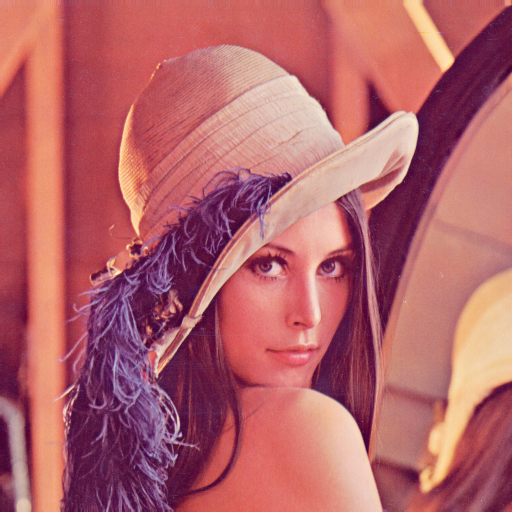
\includegraphics[width=.3\textwidth]{../examples/lena/lena.png}\quad
				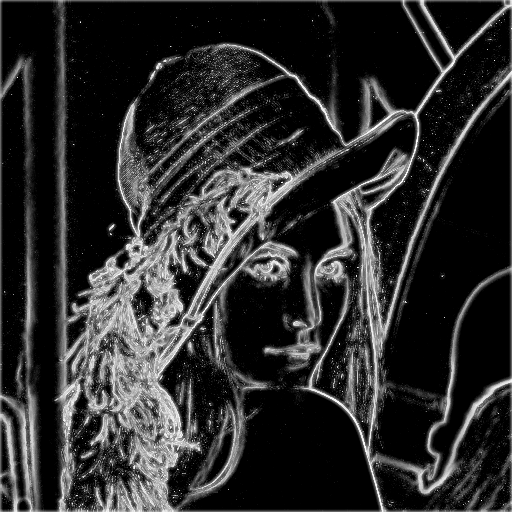
\includegraphics[width=.3\textwidth]{../examples/lena/no-geom_raw.png}\quad
				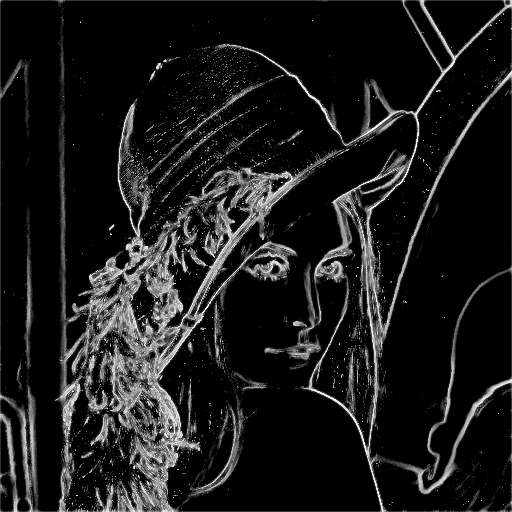
\includegraphics[width=.3\textwidth]{../examples/lena/15_out_raw.png}
				\caption{Ein Testdurchlauf mit $t=15$ und der $7\times 7$ Maske. Ganz links ist das Originalbild. In der Mitte ist $g$ die Maskengröße und rechts $\frac{3}{4}$ der Maskengröße.}
				\label{fig:lena_first_test}
			\end{figure}

			Da dieser Algorithmus von den lokalen Bedingungen jedes Pixels abhängt, kann dieser Algorithmus nicht durch eine Faltung ausgedrückt werden, wie etwa eine Reihe anderer Filter, darunter der Gaussche Filter aus \ref{sec:imageproc}, aber auch der Kantendetektor von Canny (siehe [x]).

		\subsection{Non-Maximum-Suppression}\label{ssec:nonmax}
			Das oben genannte Prinzip aus Abschnitt \ref{ssec:susan_principle} findet Kanten innerhalb von Bildern, aber die Lokalisation der Kanten könnte besser sein, wie wir in der Abbildung \ref{fig:susan_principle} bereits erkennen konnten. Im Bereich der eigentlichen Kante stellen wir fest, dass die Antwort $A$ ungleich $0$ ist. Um die Kante genauer zu lokalisieren, verwenden wir das Prinzip der Non-Maximum-Suppression, bei der nur die maximale Antwort entlang einer Kante erhalten bleibt.
			Zu diesem Zweck berechnen wir die Richtung eines jeden Pixels $r_0 = (x_0, y_0)$, für welches $A(x_0, y_0) \neq 0$ gilt, durch eine Fallunterscheidung. Wir unterscheiden dabei verschiedene Arten von Kanten.

			Der Inter-Pixel-Fall liegt vor, wenn eine Kante zwischen zwei Pixeln liegt. Der Intra-Pixel-Fall liegt vor, wenn ein Pixel genau auf der Kante liegt. In den Abbildungen stehen die grün markierten Pixel jeweils für Pixel, die in der USAN liegen. Die roten Pixel liegen außerhalb der USAN. Die Mitte ist der Nucleus der Maske.
			\begin{figure}[H]
				\begin{center}
					\begin{minipage}{0.5\textwidth}\centering
						\begin{tikzpicture}[fill=black, text=white, color=black]
							\tiny
							\matrix(m)[matrix of nodes, nodes={draw, minimum size = 0.6cm}, nodes in empty cells, column sep=-\pgflinewidth,row sep=-\pgflinewidth]{
								|[fill=white!29!black]|\phantom{H}	&|[fill=white!29!black]|\phantom{H}	&|[fill=white!29!black]|\phantom{H}	&|[fill=white!29!black]|\phantom{H}	&|[fill=white!29!black]|\phantom{H}	&|[fill=white!29!black]|\phantom{H}	&|[fill=white!29!black]|\phantom{H}	&|[fill=white!29!black]|\phantom{H}	\\ 
								|[fill=white!29!black]|\phantom{H}	&|[fill=white!29!black]|\phantom{H}	&|[fill=white!29!black]|\phantom{H}	&|[fill=white!29!black]|\phantom{H}	&|[fill=white!29!black]|\phantom{H}	&|[fill=white!29!black, text=white]|B	&|[fill=white!29!black]|\phantom{H}	&|[fill=white!29!black]|\phantom{H}	\\ 
								|[fill=white!29!black]|\phantom{H}	&|[fill=white!29!black]|\phantom{H}	&|[fill=white!29!black]|\phantom{H}	&|[fill=white!29!black]|\phantom{H}	&|[fill=white!100!black, text=black]|\phantom{H}	&|[fill=white!100!black, text=black]|A	&|[fill=white!100!black, text=black]|\phantom{H}	&|[fill=white!100!black, text=black]|\phantom{H}\\ 
								|[fill=white!29!black]|\phantom{H}	&|[fill=white!29!black]|\phantom{H}	&|[fill=white!29!black]|\phantom{H}	&|[fill=white!29!black]|\phantom{H}	&|[fill=white!100!black, text=black]|\phantom{H}	&|[fill=white!100!black, text=black]|\phantom{H}	&|[fill=white!100!black, text=black]|\phantom{H}	&|[fill=white!100!black, text=black]|\phantom{H}\\ 
								|[fill=white!100!black, text=black]|\phantom{H}	&|[fill=white!100!black, text=black]|\phantom{H}	&|[fill=white!100!black, text=black]|\phantom{H}	&|[fill=white!29!black]|\phantom{H}			&|[fill=white!100!black, text=black]|\phantom{H}	&|[fill=white!100!black, text=black]|\phantom{H}	&|[fill=white!100!black, text=black]|\phantom{H}	&|[fill=white!100!black, text=black]|\phantom{H}	\\ 
								|[fill=white!100!black, text=black]|\phantom{H}	&|[fill=white!100!black, text=black]|\phantom{H}	&|[fill=white!100!black, text=black]|\phantom{H}	&|[fill=white!29!black, text=white]|C		&|[fill=white!100!black, text=black]|\phantom{H}	&|[fill=white!100!black, text=black]|\phantom{H}	&|[fill=white!100!black, text=black]|\phantom{H}	&|[fill=white!100!black, text=black]|\phantom{H}	\\ 
								|[fill=white!100!black, text=black]|\phantom{H}	&|[fill=white!100!black, text=black]|\phantom{H}	&|[fill=white!100!black, text=black]|\phantom{H}	&|[fill=white!29!black]|\phantom{H}			&|[fill=white!100!black, text=black]|\phantom{H}	&|[fill=white!100!black, text=black]|\phantom{H}	&|[fill=white!100!black, text=black]|\phantom{H}	&|[fill=white!100!black, text=black]|\phantom{H}	\\ 
								|[fill=white!100!black, text=black]|\phantom{H}	&|[fill=white!100!black, text=black]|\phantom{H}	&|[fill=white!100!black, text=black]|\phantom{H}	&|[fill=white!29!black]|\phantom{H}			&|[fill=white!100!black, text=black]|\phantom{H}	&|[fill=white!100!black, text=black]|\phantom{H}	&|[fill=white!100!black, text=black]|\phantom{H}	&|[fill=white!100!black, text=black]|\phantom{H}	\\ 
							};				
						\end{tikzpicture}

						Eingangsbild
					\end{minipage}
					\begin{minipage}{0.45\textwidth}\centering
						\begin{tikzpicture}[fill=red]
							\tiny
							\matrix(m)[matrix of nodes, nodes={draw, minimum size = 0.5cm}, nodes in empty cells, column sep=-\pgflinewidth,row sep=-\pgflinewidth]{
								|[fill]|\phantom{H}& |[fill]|\phantom{H}& |[fill]|\phantom{H}\\
								|[fill=green]|\phantom{H}& |[fill=green]|A& |[fill=green]|\phantom{H}\\
								|[fill=green]|\phantom{H}& |[fill=green]|\phantom{H}& |[fill=green]|\phantom{H}\\
							};
						\end{tikzpicture}
						\begin{tikzpicture}[fill=red]
							\tiny
							\matrix(m)[matrix of nodes, nodes={draw, minimum size = 0.5cm}, nodes in empty cells, column sep=-\pgflinewidth,row sep=-\pgflinewidth]{
								|[fill=green]|\phantom{H}& |[fill=green]|\phantom{H}& |[fill=green]|\phantom{H}\\
								|[fill=green]|\phantom{H}& |[fill=green]|B& |[fill=green]|\phantom{H}\\
								|[fill]|\phantom{H}& |[fill]|\phantom{H}& |[fill]|\phantom{H}\\
							};
						\end{tikzpicture}

						Inter-Pixel-Fall
						\vspace{1em}

						\begin{tikzpicture}[fill=red]
							\tiny
							\matrix(m)[matrix of nodes, nodes={draw, minimum size = 0.5cm}, nodes in empty cells, column sep=-\pgflinewidth,row sep=-\pgflinewidth]{
								|[fill]|\phantom{H}& |[fill=green]|\phantom{H}& |[fill]|\phantom{H}\\
								|[fill]|\phantom{H}& |[fill=green]|C& |[fill]|\phantom{H}\\
								|[fill]|\phantom{H}& |[fill=green]|\phantom{H}& |[fill]|\phantom{H}\\
							};
						\end{tikzpicture}

						Intra-Pixel-Fall


					\end{minipage}

					\caption{Inter-Pixel-Fall und Intra-Pixel-Fall für die $3\times 3$ Maske: Die drei rechts abgebildeten USAN wurden durch wählen des Nucleus an den mit A, B und C markierten Stellen im Eingangsbild ausgewertet. Die grün markierten Pixel stehen für Teile der USAN.}
					\label{fig:inter-intra}
				\end{center}
			\end{figure}

			Wir werden zunächst jede Antwort in einen der zwei Fälle einsortieren, danach können wir die Richtung bestimmen.

			\begin{enumerate}
				\item \textbf{Inter-Pixel:}

				\noindent Falls die Größe der USAN größer ist als der Maskendurchmesser und die Distanz zwischen $\text{COG}(r_0)$ und $r_0$ größer als $1$ Pixel ist, so ist die Richtung $D(r_0)$ gegeben durch
				$$ D(r_0) = \begin{cases}
					\text{arctan}\bigg(
						\frac{x_0 - \text{COG}(x_0)}
						{y_0 - \text{COG}(y_0)}
					\bigg) & \text{falls } \text{COG}(y_0) \neq y_0 \\
					
					\frac{\pi}{2} & \text{sonst}

				\end{cases}, $$
				wobei
				$$ \text{COG}(r_0) := \frac	{\sum_r r\,c(r,r_0)}	{\sum_r c(r,r_0)} = \frac	{\sum_r r\,c(r,r_0)} {n(r_0)}$$
				das sogenannte Gravitationszentrum (\emph{center of gravity}) ist.
				\item \textbf{Intra-Pixel:}
				
				\noindent Andernfalls müssen wir die zweiten Momente der USAN folgendermaßen berechnen:
				\begin{align*}
					d_{x_0} &:= \sum_r (x-x_0)^2 \, c_t(r,r_0) \\
					d_{y_0} &:= \sum_r (y-y_0)^2 \, c_t(r,r_0) \\
					\sigma 	&:= -\text{sgn}\bigg(\sum_r (x-x_0) \, (y-y_0) \, c_t(r,r_0)\bigg)
				\end{align*}
				Dabei ergibt sich die Kantenrichtung als
				$$ D(r_0) = \begin{cases}
						\sigma \, \text{arctan} \, \frac{d_{y_0}}{d_{x_0}} 	&	\text{falls } d_{x_0} \neq 0 \\ 
						\frac{\pi}{2}										&	\text{sonst}
					\end{cases}$$
				Falls allerdings $d_{x_0} = 0$, so ist $D(r_0) = \frac{\pi}{2}$
			\end{enumerate}

			\begin{figure}[H]\centering
				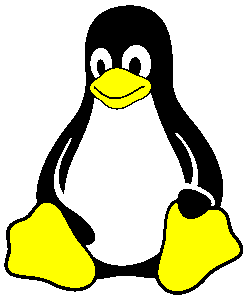
\includegraphics[width=.4\textwidth]{../examples/tux/tux.png}\quad
				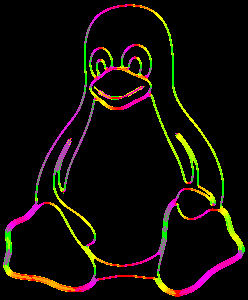
\includegraphics[width=.4\textwidth]{../examples/tux/15_out_heat.png}\quad
				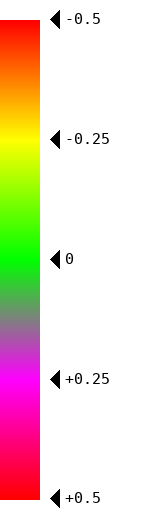
\includegraphics[width=.14\textwidth]{assets/heatmap-strip/strip.png}
				\caption{Ein Testdurchlauf für das Berechnen der Richtungen mit $t=15$. Links ist das Eingangsbild. Rechts ist die Kantenrichtung für jedes Pixel abgebildet. Die Zahlenwerte können an der Skala abgelesen werden und sind als Vielfache von $\pi$ angegeben.}
				\label{fig:directions_test}
			\end{figure}

			Die Berechnungen für die jeweiligen Kantenrichtungen an jedem Pixel werden in der Implementation gleichzeitig mit den Berechnungen für das SUSAN-Prinzip durchgeführt. Auf diese Weise müssen $c_t$ und $n$ an jeder Stelle nur einmal berechnet werden.

			\begin{figure}[H]\centering
				\begin{tikzpicture}[fill=black, text=white]
					\tiny
					\matrix(m)[matrix of nodes, nodes={draw, minimum size = .6cm}, column sep=-\pgflinewidth,row sep=-\pgflinewidth]{
						|[fill=white!57!black]|147	&|[fill=white!15!black]|40	&|[fill=white!15!black]|40	&|[fill=white!15!black]|40	&|[fill=white!57!black]|147	&|[fill=white!100!black, text=black]|255	&|[fill=white!57!black]|147	&|[fill=white!15!black]|40	&|[fill=white!15!black]|40	&|[fill=white!15!black]|40	&|[fill=white!57!black]|147	\\ 
						|[fill=white!15!black]|40	&|[fill=white!0!black]|0	&|[fill=white!0!black]|0	&|[fill=white!0!black]|0	&|[fill=white!0!black]|0	&|[fill=white!78!black, text=black]|201	&|[fill=white!0!black]|0	&|[fill=white!0!black]|0	&|[fill=white!0!black]|0	&|[fill=white!0!black]|0&|[fill=white!15!black]|40	\\ 
						|[fill=white!15!black]|40	&|[fill=white!0!black]|0	&|[fill=white!0!black]|0	&|[fill=white!0!black]|0	&|[fill=white!0!black]|0	&|[fill=white!78!black, text=black]|201	&|[fill=white!0!black]|0	&|[fill=white!0!black]|0	&|[fill=white!0!black]|0	&|[fill=white!0!black]|0&|[fill=white!15!black]|40	\\ 
						|[fill=white!15!black]|40	&|[fill=white!0!black]|0	&|[fill=white!0!black]|0	&|[fill=white!0!black]|0	&|[fill=white!0!black]|0	&|[fill=white!78!black, text=black]|201	&|[fill=white!0!black]|0	&|[fill=white!0!black]|0	&|[fill=white!0!black]|0	&|[fill=white!0!black]|0&|[fill=white!15!black]|40	\\ 
						|[fill=white!15!black]|40	&|[fill=white!0!black]|0	&|[fill=white!0!black]|0	&|[fill=white!0!black]|0	&|[fill=white!0!black]|0	&|[fill=white!78!black, text=black]|201	&|[fill=white!0!black]|0	&|[fill=white!0!black]|0	&|[fill=white!0!black]|0	&|[fill=white!0!black]|0&|[fill=white!15!black]|40	\\ 
						|[fill=white!15!black]|40	&|[fill=white!0!black]|0	&|[fill=white!0!black]|0	&|[fill=white!0!black]|0	&|[fill=white!0!black]|0	&|[fill=white!78!black, text=black]|201	&|[fill=white!0!black]|0	&|[fill=white!0!black]|0	&|[fill=white!0!black]|0	&|[fill=white!0!black]|0&|[fill=white!15!black]|40	\\ 
						|[fill=white!15!black]|40	&|[fill=white!0!black]|0	&|[fill=white!0!black]|0	&|[fill=white!0!black]|0	&|[fill=white!0!black]|0	&|[fill=white!78!black, text=black]|201	&|[fill=white!0!black]|0	&|[fill=white!0!black]|0	&|[fill=white!0!black]|0	&|[fill=white!0!black]|0&|[fill=white!15!black]|40	\\ 
						|[fill=white!15!black]|40	&|[fill=white!0!black]|0	&|[fill=white!0!black]|0	&|[fill=white!0!black]|0	&|[fill=white!0!black]|0	&|[fill=white!78!black, text=black]|201	&|[fill=white!0!black]|0	&|[fill=white!0!black]|0	&|[fill=white!0!black]|0	&|[fill=white!0!black]|0&|[fill=white!15!black]|40	\\ 
						|[fill=white!15!black]|40	&|[fill=white!0!black]|0	&|[fill=white!0!black]|0	&|[fill=white!0!black]|0	&|[fill=white!0!black]|0	&|[fill=white!78!black, text=black]|201	&|[fill=white!0!black]|0	&|[fill=white!0!black]|0	&|[fill=white!0!black]|0	&|[fill=white!0!black]|0&|[fill=white!15!black]|40	\\ 
						|[fill=white!15!black]|40	&|[fill=white!0!black]|0	&|[fill=white!0!black]|0	&|[fill=white!0!black]|0	&|[fill=white!0!black]|0	&|[fill=white!78!black, text=black]|201	&|[fill=white!0!black]|0	&|[fill=white!0!black]|0	&|[fill=white!0!black]|0	&|[fill=white!0!black]|0&|[fill=white!15!black]|40	\\ 
						|[fill=white!57!black]|147	&|[fill=white!15!black]|40	&|[fill=white!15!black]|40	&|[fill=white!15!black]|40	&|[fill=white!57!black]|147	&|[fill=white!100!black, text=black]|255	&|[fill=white!57!black]|147	&|[fill=white!15!black]|40	&|[fill=white!15!black]|40	&|[fill=white!15!black]|40	&|[fill=white!57!black]|147	\\ 
					};
					\normalsize
				\end{tikzpicture}
				\caption{Eingangsbild wie in Abbildung \ref{fig:susan_principle}. Durch die Non-Maximum-Suppression wurde die Kante pixelgenau lokalisiert}
			\end{figure}

			Die Richtung lohnt sich nur für diejenigen Pixel $(i,j)$ zu bestimmen, für die $A(i,j) > 0$ gilt. Ist die Richtung der Kante bestimmt, so können wir die lokalen Maxima von $A$ entlang der Richtung, die senkrecht zur Kantenrichtung steht, erhalten. Alles, was kein lokales Maximum entlang dieser Richtung ist, wird verworfen. Wir erhalten so ein neues Bild. In Kapitel \ref{sec:implementation} wird darauf eingegangen, wie genau dieser Prozess implementiert wurde.

			Die Non-Maximum-Suppression unterdrückt in unserem Beispiel tatsächlich alle diejenigen Pixel, die keine lokalen Maxima in der Richtung senkrecht zur Kante sind. Auch für größere Bilder erzielt die Non-Maximum-Suppression den erwünschten Effekt, siehe Abbildung \ref{fig:lena_nonmax_supp}.

			\begin{figure}[H]\centering
				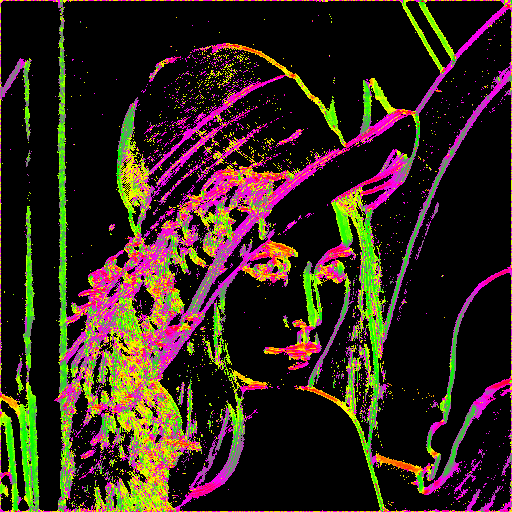
\includegraphics[width=.3\textwidth]{../examples/lena/15_out_heat.png}\quad
				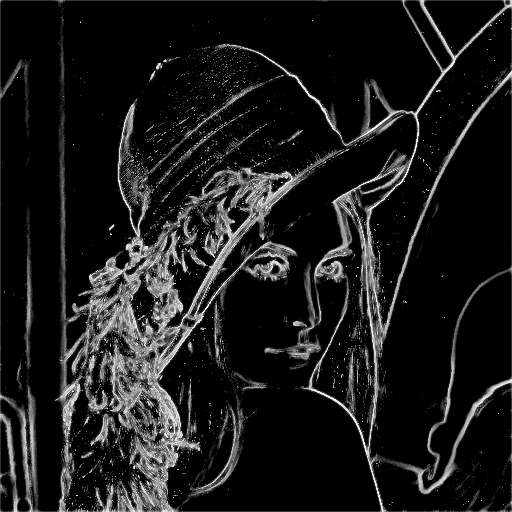
\includegraphics[width=.3\textwidth]{../examples/lena/15_out_raw.png}\quad
				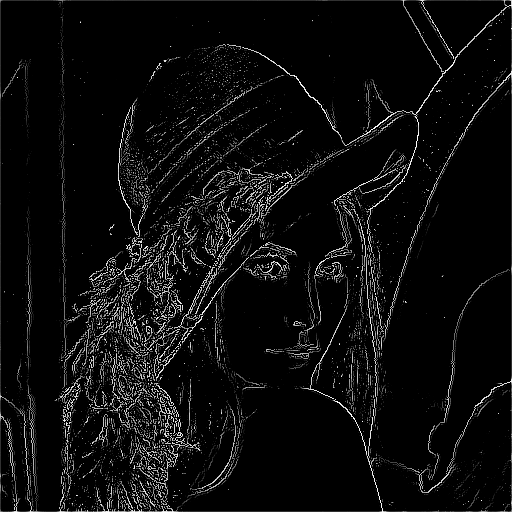
\includegraphics[width=.3\textwidth]{../examples/lena/15_out_nonmax_supp.png}

				\caption{Wie Abbildung \ref{fig:lena_first_test}. Links das Bild mit den Kantenrichtungen (Skala wie in Abbildung \ref{fig:directions_test}). In der Mitte das Bild nach dem prinzipiellen SUSAN-Schritt. Das Bild rechts ist nach der Non-Maximum-Suppression.}
				\label{fig:lena_nonmax_supp}
			\end{figure}


		\subsection{Ausdünnen}\label{ssec:thinout}
			Da viele digitale Bilder eingangs mit Rauschen behaftet sind, ist es manchmal hilfreich, einzelne Antworten zu entfernen und dafür andere hinzuzufügen. Zu diesem Zwecke empfiehlt \cite{SUSAN}, dass man einige der Kanten ausdünnt. Dieser Vorgang wird genauer in \cite{thinout} beschrieben.
			Es wird erneut über das ganze Bild iteriert. Jedes Pixel $(i,j)$ mit einer Antwort $A(i,j) > 0$ wird auf die Anzahl seiner direkten Nachbarn mit $A(x,y) > 0$ überprüft. Als direkte Nachbarschaft werden die acht nächsten Pixel bezeichnet, siehe dazu die $3\times 3$ Maske in Abbildung \ref{fig:def_masken}. Angenommen, das Pixel hat...
			\begin{itemize}
				\item \textbf{0 Nachbarn:}
					Entferne die Antwort des Pixels.
				\item \textbf{1 Nachbar:}
					Überprüfe, ob in einer Reichweite von 3 Pixeln eine Linie mit der gleichen Richtung existiert. Falls ja, verbinde die Pixel miteinander.
				\item \textbf{2 Nachbarn:}
					Falls das Pixel adjazent zu einer diagonalen Linie ist, entferne es.
					Falls das Pixel außerhalb einer sonst horizontalen oder vertikalen Linie liegt, verschiebe die Antwort des Pixels in die Lücke der vertikalen oder horizontalen Linie
				\item \textbf{3 Nachbarn:}
					Falls die drei Nachbarn in einer Linie liegen, entferne die Antwort des Pixels.
			\end{itemize}

			Im Testbild der Abbildung \ref{fig:thinout_test} erkennt man die Funktionsweise in allen vier oben genannten Fällen.

			\begin{figure}[H]\centering
				
\includegraphics[width=0.45\textwidth]{./assets/thinout/out_nonmax_supp.png}\quad
				
\includegraphics[width=0.45\textwidth]{./assets/thinout/out_thinned.png}

				\vspace{0.5em}

				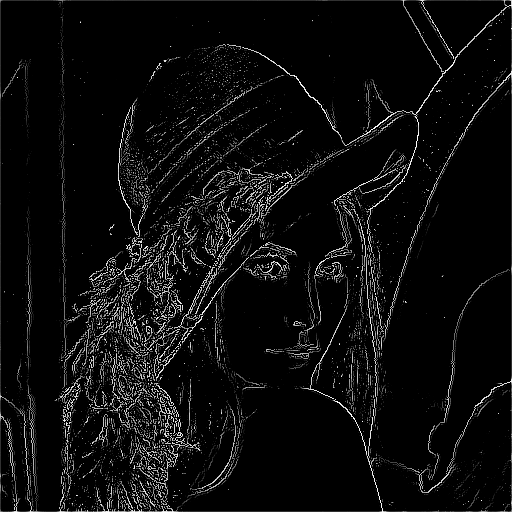
\includegraphics[width=0.45\textwidth]{../examples/lena/15_out_nonmax_supp.png}\quad
				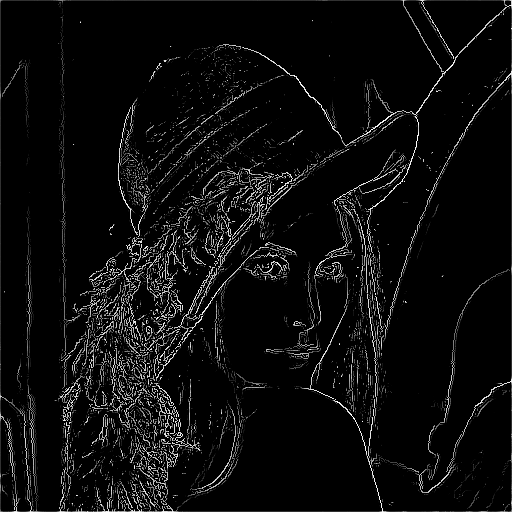
\includegraphics[width=0.45\textwidth]{../examples/lena/15_out_thinned.png}
				\caption{Links: Kantenbilder nach der Non-Maximum-Suppression. Rechts: Kantenbilder nach dem Ausdünnen.}
				\label{fig:thinout_test}
			\end{figure}


		\subsection{Der SUSAN-Eckendetektor}\label{ssec:corner_detector}
			In \cite{SUSAN} wird zusätzlich ein Verfahren beschrieben, mit welchem sich durch das SUSAN-Prinzip Ecken finden lassen. Dieser Eckendetektor basiert darauf, dass der SUSAN Kantendetektor an Ecken stärkere Antworten liefert als an Kanten. Man verwendet also im ersten Schritt des Eckendetektors lediglich einen niederigeren Wert für $g$ in \ref{sec:thealgorithm}.
			Danach finden sich immer noch viele falsch positive Antworten. Um diese zu vermeiden, überprüft man, ob die jeweiligen Kandidaten mit einer Kante zusammenhängen. Dies gelingt durch das Erzwingen folgender Regeln für jede Ecke:

			\begin{enumerate}
				\item Die Entfernung zwischen Gravitationszentrum und Nucleus muss groß genug sein
				\item Jedes Pixel in der Maske, welches sich auf gerader Strecke zwischen Nucleus und Gravitationszentrum befindet, muss in der USAN des Nucleus enthalten sein.
				\item Alles, was kein lokales Maximum in einer $5\times 5$ Maske ist, soll entfernt werden. 
			\end{enumerate}

			Die Entfernung zwischen Gravitationszentrum und Nucleus versichert, dass die Richtung der Kante sich an der Ecke ändert. Punkt garantiert den räumlichen Zusammenhang von Ecken und Kanten. Der dritte Punkt ist vom Prinzip gleich der Non-Maximum-Suppression.

			\begin{figure}[H]\centering
				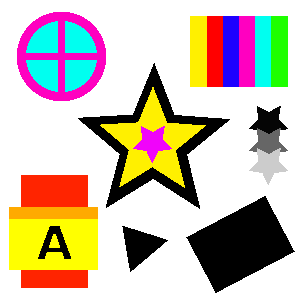
\includegraphics[width=0.45\textwidth]{../examples/original/original.png}\quad
				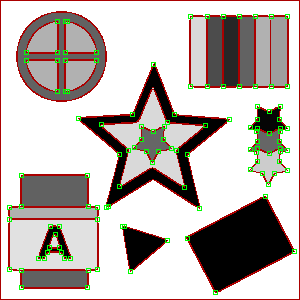
\includegraphics[width=0.45\textwidth]{../examples/original/test_overlay.png}
				\caption{Die Ecken sind grün umrahmt wohingegen die Kanten rot übergezeichnet sind.}
				\label{fig:corner_test}
			\end{figure}

		\section{Implementation}\label{sec:implementation}
		Meine persönliche Implementation ist in Python 3 erfolgt. Die Software ist abhängig von den folgenden Python 3 Paketen:
		\begin{itemize}
			\item \texttt{pillow}, eine Bibiliothek für Bildverarbeitung \cite{pillow}
			\item \texttt{numpy}, eine Bibliothek für wissenschaftliches Rechnen \cite{numpy}
			\item \texttt{multiprocessing} eine Bibiliothek für prozessbasierte Parallelisierung  \cite{multiprocessing}
		\end{itemize}
		Die Software ist verfügbar unter dem Link \texttt{https://gitlab.gwdg.de/julian.lueken/susan/}. In der Klasse \texttt{Susan.py} befindet sich der vollständige Kantendetektor. Er lässt sich per \texttt{import Susan} nutzen. Dazu erzeugt man ein Objekt der \texttt{Susan}-Klasse und übergibt eine Bilddatei. Danach ruft man auf dem Objekt die Funktion \texttt{detect\_edges\_mp} mit dem Parameter $t$, dem Grenzwert aus Abschnitt \ref{ssec:susan_principle}, auf.

		\begin{figure}[H] \centering
			\begin{lstlisting}[language=Python]
				import Susan

				t = 15
				S = Susan("lena.png")
				S.detect_edges_mp(t)
			\end{lstlisting}
		\caption{Nutzen der Python 3 Applikation}
		\label{fig:minimal-working-example}
		\end{figure}

		Es können weiterhin folgende Parameter übergeben werden:
		\begin{center}
			\begin{tabular}{|l|l|l|l|}
				\hline
				\textbf{Name} 		& \textbf{Beschreibung} 	& \textbf{Datentyp}							& \textbf{Standardwert}	\\
				\hline
				\texttt{t}			& Grenzwert	für $c_t$		& Ganzzahl, $t \in [1,255]_\mathbb{N}$		& -\\
				\hline
				\texttt{filename}	& Ausgabepfad				& Zeichenkette								& \texttt{"{}out.png"}\\
				\hline
				\texttt{nms}		& Non-Maximum-				& Boolesch									& \texttt{True}\\
									& Suppression & & \\
				\hline
				\texttt{heatmap}	& Ausgabe der Richtungen 	& Boolesch									& \texttt{False}\\
				\hline
				\texttt{geometric}	& Schwache Antworten 		& Boolesch 									& \texttt{True} \\
									& unterdrücken & & \\
				\hline
				\texttt{corners}	& Ecken finden				& Boolesch									& \texttt{False} \\
				\hline
				\texttt{overlay}	& Überlagerungsbild 		& Boolesch									& \texttt{True} \\
									& erzeugen & & \\
				\hline
			\end{tabular}
		\end{center}

		Beim Paramater \texttt{heatmap} werden die Richtungen als Bild ausgegeben, dabei korrespondieren die Richtungen zu Farben, genau so wie wir es schon in den Abbildungen zu Abschnitt \ref{ssec:nonmax} sehen konnten.
		Falls \texttt{geometric} auf \texttt{True} gesetzt ist, so wird $g$ als $\frac{3}{4}$ der Maskengröße gewählt. Andernfalls ist $g$ gleich der Maskengröße, wie im Abschnitt \ref{ssec:susan_principle}.
		Die Option \texttt{overlay} erzeugt ein Bild, auf dem Kanten in rot nachgezeichnet und Ecken von grünen Kästen umrahmt werden, wie in Abbildung \ref{fig:corner_test}.

			\subsection{Vergleichsfunktion}
				Zu Gunsten der Effizienz habe ich für die Vergleichsfunktion eine Lookup-Tabelle implementiert, wie es auch in [quelle] nahgelegt wurde. Beim Initialisieren des \texttt{Susan}-Objekts wird ein Feld erzeugt. Das Ziel ist es, alle möglichen Werte, die $c_t$ (siehe \ref{ssec:susan_principle}) annehmen kann, zu speichern.
				In unserem Fall ist $c_t$ folgendermaßen definiert:
				
				$$
					c_t(a,b) :=
						\text{exp}\left(-\left(\frac{I(a) - I(b)}{t}\right)^6\right)
				$$
				
				Ein Pixel in einem 8-bit Graustufenbild kann $2^8 = 256$ mögliche Intensitäten annehmen, demnach braucht das Feld für die Differenz zweier solcher Graustufenintensitäten $512$ Plätze.
				Regulär werden Felder entweder ab $0$ oder $1$ indiziert. In Python werden Felder ab $0$ indiziert, allerdings bietet Python den Vorteil, dass man mit Index $-i$ das $i$-te Element von hinten abrufen kann. In der Implementation ist diese Lookup-Tabelle dank dieser speziellen Art der Indizierung einfach und elegant: Der Index $a-b$ des Feldes steht für $c_t(a,b)$.

			\subsection{Non-Maximum-Suppression}
				Die Non-Maximum-Suppression ist ein Vorgang, bei der jede Kante genauer lokalisiert wird. Entlang einer Kante soll immer nur die maximale Antwort erhalten bleiben.
				Um die Non-Maximum-Suppression durchzuführen, wird zunächst für jedes Pixel $(i,j)$ mit $A(i,j) > 0$ die Kantenrichtung $D(i,j)$ bestimmt. Die möglichen Kantenrichtungen werden dann für einen Zwischenschritt kategorisiert. Die Kategorien sind \emph{negativ diagonal}, \emph{vertikal}, \emph{positiv diagonal} und \emph{horizontal}. Die Kategorie bestimmt, welche zwei adjazenten Pixel $C$ für die Non-Maximum-Suppression interessant sind.
				\begin{center}
					\begin{tabular}{|ll|l|ll|}
					\hline
					\textbf{Bedingung}					&								& \textbf{Kategorie}			& \textbf{Adjazente $C$} 	&	\\
					\hline
														&$D(i,j) \leq -\frac{3}{8}\pi$ 	& negativ diagonal 				&$\{(i+1, j-1)$, 		&$(i-1, j+1)\}$\\
					\hline
					$D(i,j) > -\frac{3}{8}\pi$, 		&$D(i,j) \leq -\frac{1}{8}\pi$ 	& horizontal 					&$\{(i-1, j)$, 			&$(i+1, j)\}$\\
					\hline
					$D(i,j) > -\frac{1}{8}\pi$, 		&$D(i,j) \leq \frac{1}{8}\pi$ 	& positiv diagonal 				&$\{(i+1, j+1)$, 		&$(i-1, j-1)\}$\\
					\hline
					$D(i,j) > -\frac{3}{8}\pi$			&								& vertikal						&$\{(i, j-1)$, 			&$(i, j+1)\}$\\
					\hline
					\end{tabular}
				\end{center}
				Für jedes Pixel $(i,j)$ wird nun überprüft, ob $(i,j) = \text{max}(C \cup \{(i,j)\})$ gilt. Gilt es nicht, so wird $A(i,j)$ unterdrückt.
				
			\subsection{Parallelisierung}
				Das SUSAN-Prinzip sieht vor, die Antwort $A(i,j)$ und die Kantenrichtung $D(i,j)$ aus  immer nur mithilfe von Pixeln aus der Maske auf $(i,j)$ zu berechnen. An dieser Stelle kann die Berechnung von $A$ und $D$ parallelisiert werden. In meiner Implementation liefert das Paket \texttt{multiprocessing} die nötigen Werkzeuge, um die vorhandenen Ressourcen zusammenzuschließen und die Berechnung von $A$ und $D$ parallel abzuarbeiten.

				Der Einfachheit halber habe ich das Bild nur der Höhe nach partitioniert. Eine Partitionierung $\mathcal{S}$ ist eine Menge von nichtnegativen ganzen Zahlen $\{S_1, S_2, ..., S_n, S_{n+1}\}$. Für alle $i \in \{1,2,...,n\}$ arbeitet der Job $J_i$ die Partition $(S_i, S_{i+1}]_\mathbb{Z}$ ab.

				Unter der stark vereinfachten Annahme, dass alle Kerne gleich viele Fließkommazahloperationen pro Zeiteinheit abarbeiten können und gleichgroße Partitionen etwa gleichviel Rechenzeit benötigen, gelte folgende Aussage: Eine Partitionierung $\mathcal{S}$ für die gilt $\#\mathcal{S} = n+1$ ist genau dann optimal, wenn für alle Partitionen gilt
				$$|\#(S_i, S_{i+1}]_\mathbb{Z} - \#(S_j, S_{j+1}]_\mathbb{Z}| \leq 1, \quad \forall i \neq j, \quad i,j \in \{1,2,...,n\}$$

				Angenommen der Computer, auf dem die Software läuft, besitzt $n$ Kerne, kann also $n$ Jobs $J_1,J_2,...,J_n$ gleichzeitig abarbeiten, und ein Bild der Höhe $H$ wird eingegeben. Sei $k := H \text{ mod } n$ und $z := \left\lfloor \frac{H}{n} \right\rfloor$. Dann ist die optimale Partitionierung $\mathcal{S}$ nach der Höhe gegeben durch:

				\begin{align*}
				S_1 	&= 					0		\\
				S_2 	&= S_1		+	z + 1		\\
				S_3 	&= S_2 		+ 	z + 1		\\
									\vdots			\\
				S_{k-1} &= S_{k-2}	+ 	z + 1		\\
				S_{k}	&= S_{k-1} 	+ 	z + 1		\\
				S_{k+1} &= S_k 		+ 	z			\\
									\vdots			\\
				S_{n} 	&= S_{n-1} 	+ 	z 			\\
				S_{n+1} &= S_{n}	+	z  = H	\\
				\end{align*}

				Die Jobs $J_1, J_2, ..., J_n$ arbeiten das komplette Bild ab, denn es gilt

				$$ \bigcup_{i=1}^n \left(S_i, S_{i+1}\right]_\mathbb{Z} = (0,H]_\mathbb{Z} = [1,H]_\mathbb{Z} $$

		
		\section{Numerische Experimente}
			\subsection{Variation des Grenzwerts}
			\subsection{Vergleich mit dem Kantendetektor von Canny}
				In diesem Abschnitt wird der Kantendetektor von Canny [x] kurz vorgestellt und anschließend mit dem SUSAN-Kantendetektor verglichen. Der Kantendetektor von Canny basiert auf dem Prinzip der Ableitung: Ziel ist es, die Stellen der größten Änderung zu markieren. In der stetigen Analysis sind diese Stellen die Nullstellen der zweiten Ableitung. Da wir allerdings keine stetige Funktion vorliegen haben, sondern lediglich ein digitales Bild, müssen wir eine Approximation finden.

				Zunächst aber wird das Bild geglättet, meist durch einen Gausschen Weichzeichner, wie er bereits in [x] besprochen wurde.

				Unter den Begriff Sobel-Operator fallen Filtermasken, die eine Approximation der ersten Ableitung in eine Richtung berechnen und orthogonal dazu das Bild glätten.

				Mit den Sobel-Operatoren $S_x$ und $S_y$ lassen sich die geglätteten Approximationen der partiellen Ableitungen folgendermaßen berechnen
				$$ g_x = S_x * I \qquad g_y = S_y * I, $$
				wobei 
			 	$$ S_x = \begin{pmatrix}
			 		-1 & 0 & 1\\
			 		-2 & 0 & 2\\
			 		-1 & 0 & 1\\
			 	\end{pmatrix} \qquad
			 	 S_y = \begin{pmatrix}
			 		1 & 2 & 1 \\
			 		0  & 0  & 0  \\
			 		-1  & -2  & -1
				\end{pmatrix}.
				$$
				Danach werden die beiden beiden gefalteten Bilder folgendermaßen addiert
				$$ O(i,j) = |g_x(i,j) + g_y(i,j)|. $$
				Weiterhin wird, ähnlich wie beim SUSAN-Kantendetektor, eine Non-Maximum-Suppression durchgeführt. Die Kantenrichtung ist durch 
				$$ \varphi(i,j) = \begin{cases}
					\text{arctan}\bigg(
						\frac{g_y(i,j)}
						{g_x(i,j)}
					\bigg) & \text{falls } g_x(i,j) \neq 0 \\
					
					\frac{\pi}{2} & \text{sonst}

				\end{cases}, $$
				bestimmt.

				Zum Vergleich mit meiner Implementation des SUSAN-Kantendetektors ziehen wir nun die OpenCV-Implementation des Canny-Kantendetektors heran. Durch die Vektorisierbarkeit der Teilschritte lässt sich über Cannys Kantendetektor sagen, dass die Implementation in Python 3 schnellere Laufzeiten mit sich bringt. Nichtlineare Operationen müssen in Python 3, wie in den meisten anderen Programmiersprachen, über Schleifen geregelt werden. Diese sind verglichen langsam zu beispielsweise der Programmiersprache C. Das liegt begründet im dynamischen Charakters von Python \cite{pyslow}.

				Für lineare Probleme ist die Vektorisierung ein Weg, die Dynamik Pythons auszunutzen, um Ergebnisse schnell zu berechnen. Der nichtlineare Charakter des SUSAN-Detektors lässt allerdings nur einfache Parallelisierungen zu, keine Vektorisierung.

				Allerdings bringt der SUSAN-Kantendetektor einen besonders großen Vorteil mit sich. Cannys Kantendetektor findet nämlich im Gegensatz zum SUSAN-Kantendetektor keine Ecken, wie auch bereits in \cite{SUSAN} beschrieben wird.

				\begin{figure}[H]\centering
					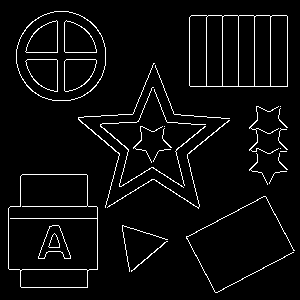
\includegraphics[width=.45\textwidth]{../examples/original/original-canny.png}\quad
					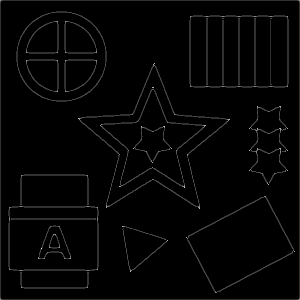
\includegraphics[width=.45\textwidth]{../examples/original/test_nonmax_supp.png}
					\caption{Links: Canny, Rechts: SUSAN.}
					\label{fig:canny_no_corners}
				\end{figure}

			\subsection{Der Eckendetektor}
			

		\section{Heuristik}
			\subsection{Erklärung des SUSAN-Prinzips}
				Für diese Heuristik nehmen wir an, dass das Bild eingangs eine stetige Funktion $I: \mathbb{R}\to \mathbb{R}$ ist.
				Der SUSAN-Kantendetektor beruht auf folgendem Prinzip: Für einen Schwellwert $t$ gibt es, abhängig von der spezifischen Stelle im Bild $x_0$ eine untere Grenze $x_0+a(x_0)$ und eine obere Grenze $x-b(x_0)$ der USAN.
				Dann gilt an den Grenzen:
				\begin{align*}
					I(x_0 + a(x_0)) &= I(x_0) + t \\
					I(x_0 - b(x_0)) &= I(x_0) - t.
				\end{align*}
				Das Prinzip des SUSAN-Kantendetektors lässt sich folgendermaßen formulieren: An genau den Stellen, an denen $n(x_0) = a(x_0) + b(x_0)$ ein Minimum hat, ist die Antwort $A(x_0) > 0$. Wir erhalten unter der Annahme, dass $n$ an $x_0$ ein lokales Minimum erreicht:
				$$ n'(x_0) = a'(x_0) + b'(x_0) = 0 $$
				Die obigen Gleichungen können wir nach $a$ und $b$ umstellen. So erhalten wir
				\begin{align*}
					a(x_0) = x_0 - x(I(x_0) + t) \\
					b(x_0) = x(I(x_0) - t) - x_0,
				\end{align*}
				wobei $x$ die Position ist.
				Damit ist $n(x_0) = x(I(x_0) + t) - x(I(x_0) - t)$ und daraus folgt
				$$ n'(x_0) = x'(I(x_0) + t) \cdot I'(x_0) - x'(I(x_0) - t) \cdot I'(x_0) = 0,$$
				anders formuliert,
				$$ x'(I(x_0) + t) \cdot I'(x_0) = x'(I(x_0) - t) \cdot I'(x_0) $$
				und damit $$x'(I(x_0) + t) = x'(I(x_0) - t),$$
				falls die Bildfunktion nicht konstant ist.
	 			Es folgt 
	 			$$(I(x_0) + t)' = (I(x_0) - t)'.$$
	 			Lassen wir $t$ gegen Null laufen, so finden wir
	 			$$\lim_{t\to 0}\; (I(x_0) + t)' - (I(x_0) - t)' = I''(x_0) = 0. $$

	 			Demnach treffen sich die maximale Antwort des SUSAN-Kantendetektors und die zweite Ableitung der Bildfunktion. Es sei dazu gesagt, dass jegliche Ableitungen nur zum Zwecke der Demonstration dienen. Im tatsächlichen SUSAN-Kantendetektor wird keine Ableitung auf dem diskreten Bild berechnet.

	 		\subsection{Berechnung der Richtungen}
	 			Die Berechnungen für die Kantenrichtungen funktionieren folgendermaßen. Im Intra-Pixel Fall schaut man sich die Umgebung des Pixels $r_0$ an und bestimmt daraus $\text{COG}(r_0)$. Im Falle einer $3\times 3$ Maske ist durch die Bedingung Intra-Pixel Bedingung gegeben, dass $n(r_0) \leq 2\cdot1.4=2.8$. 

\begin{thebibliography}{56}

\bibitem{SUSAN}
	Stephen M. Smith, J. Michael Brady,
	\textit{SUSAN - A New Approach to Low Level Image Processing},
	International Journal of Computer Vision 23(1), 45-78,
	1997

\bibitem{thinout}
	Stephen M. Smith
	\textit{Edge Thinning Used in the SUSAN Edge Detector}
	Technical Report TR95SMS5
	1995

\bibitem{gaussianblur}
	Robert Fisher, Simon Perkins, Ashley Walker, Erik Wolfart,
	\textit{Gaussian Smoothing},
	The Hypermedia Image Processing Reference 2,
	2004
	
\bibitem{pillow}
	Pillow: the friendly PIL fork, \\
	\texttt{https://python-pillow.org/}

\bibitem{numpy}
	NumPy, \\
	\texttt{https://numpy.org/}

\bibitem{multiprocessing}
	multiprocessing - Process-based parallelism, \\
	\texttt{https://docs.python.org/3/library/multiprocessing.html}

\bibitem{pyslow}
	Why Python is Slow: Looking Under the Hood
	\texttt{https://jakevdp.github.io/blog/2014/05/09/why-python-is-slow/}

\bibitem{pyparallel}
	Vectorization and parallelization in Python with NumPy and Pandas
	\texttt{https://datascience.blog.wzb.eu/2018/02/02/vectorization-and-parallelization-in-python-with-numpy-and-pandas/}
\end{thebibliography}
			


% zu den quellen:
%
% blabla überschreitet den rahmen dieser arbeit (weiterführende literatur)
% beobachtungen zum vergleich
% grundlagen
% paper auf denen meine arbeit basiert xD

\end{document}
